\documentclass{article}
\usepackage[utf8]{inputenc}

\title{TwitterBot Report}
\author{Bastien LUCAS, Rémy GAUDRU}
\date{Juin 2020}

\usepackage{natbib}
\usepackage{graphicx}

\begin{document}

\maketitle

\section{Introduction}
Le réseau social Twitter propose une API publique, permettant de publier et analyser les tweets, ouvrant la possibilité de programmer un bot (système de publication ou réponse automatique). 
\newline
\newline
Un bot rudimentaire peut permettre de tweeter régulièrement de manière programmatique, ou inversement de répondre à des tweets. Un exemple de service permettant de mettre en place en bot sans aucune connaissance en programmation est Cheap Bots Done Quick. Nous allons dans ce projet écrire une application permettant d’effectuer des analyses sur Twitter, et de mettre en place des bots très simples.

\begin{figure}[h!]
\centering

\includegraphics[scale=0.5]{images/icon.jpg}
\caption{Icone application}
\label{fig:Icone application}
\end{figure}

\section{Architecture}
Le code de l'application \textbf{twitterbot} est divisé 4 parties :
\begin{itemize}
\item 	\textbf{assets}, ce dossier contient toutes les ressources de l'application. En l'occurrence ici, le dossier contient toutes les images utilisées dans \textbf{twitterbot} comme l'icône de l'application par exemple.
\item 	\textbf{API}, ce dossier contient les fonctions appelant l'API twitter. De cette manière nous avons séparé au mieux le code de l'interface de l'application et les appels aux services de twitter, ainsi une possible modification dans le futur de l'API ou bien même de l'interface sera plus aisée.
\item 	\textbf{Components}, ce dossier contient tout le code l'interface de l'application, celui-ci est aussi découpé en 3 sous-dossiers représentant chacun une partie de l'application (Stats, Bots, Paramètres). Ainsi, chaque partie de \textbf{twitterbot} peut-être développé indépendamment les unes des autres.
\item 	\textbf{Store}, ce dossier gère le store global de l'application grâce à la librairie javascript \textbf{Redux}
\end{itemize}



\begin{figure}[h!]
\centering
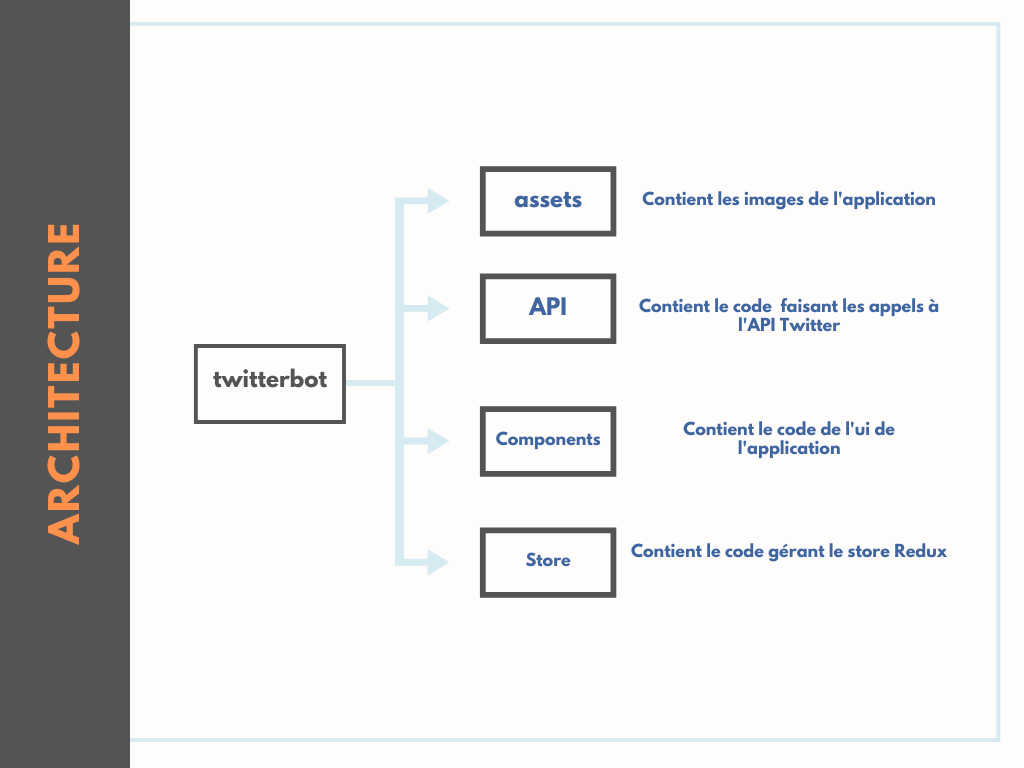
\includegraphics[scale=0.5]{images/architecture.png}
\caption{Architecture application}
\label{fig:Architecture application}
\end{figure}


\section{Développement (problèmes, solutions)}
L'utilisateur peut créer deux types de bot différents, l'un permet de poster un tweet à intervalle régulier, l'autre permet de répondre automatiquement lorqu'on le mentionne sur twitter (@BotName).
L'utilisateur pourra créer autant de bot qu'il le souhaite, pour cela il retrouvera la liste des bots créer dans le menu. Chaque bot possèdera alors un nom (choisi lors de sa création) et une image donnée alétoirement à l'aide de l'API avatars.adorable.io \citep{adorableio}

\subsection{Développement des bots (réalisé par Rémy G.)}

\subsubsection{Bot de post automatique}

Lors de la création d'un bot de post automatique, l'utilisateur peut remplir plusieurs champs. Le nom permettra de retrouver facilement son bot dans la liste des bots créés, le message du tweet sera toujours le même, cependant l'utilisateur a le choix d'afficher l'heure ou non dans son tweet. Le tweet sera alors au format [hh:mm] <message>. Afin de déterminer à quelle interval le tweet sera posté, l'utilisateur choisi parmi les 6 choix possibles (1, 5, 15, 50, 60 minutes ou 24h) dans la liste prévu à cet effet.
\newline\newline
Afin de lancer son bot, l'utilisateur clique sur celui qu'il souhaite dans la liste, un écran récapitulant les informations du bot apparaîtront, puis le lance en appuyant sur le bouton "GO". Une animation se lance indiquant à l'utilisateur que le bot est lancé. L'API twitter est alors appelée toutes les X minutes avec les paramètres choisies par l'utilisateur.

\begin{figure}[h!]
\centering
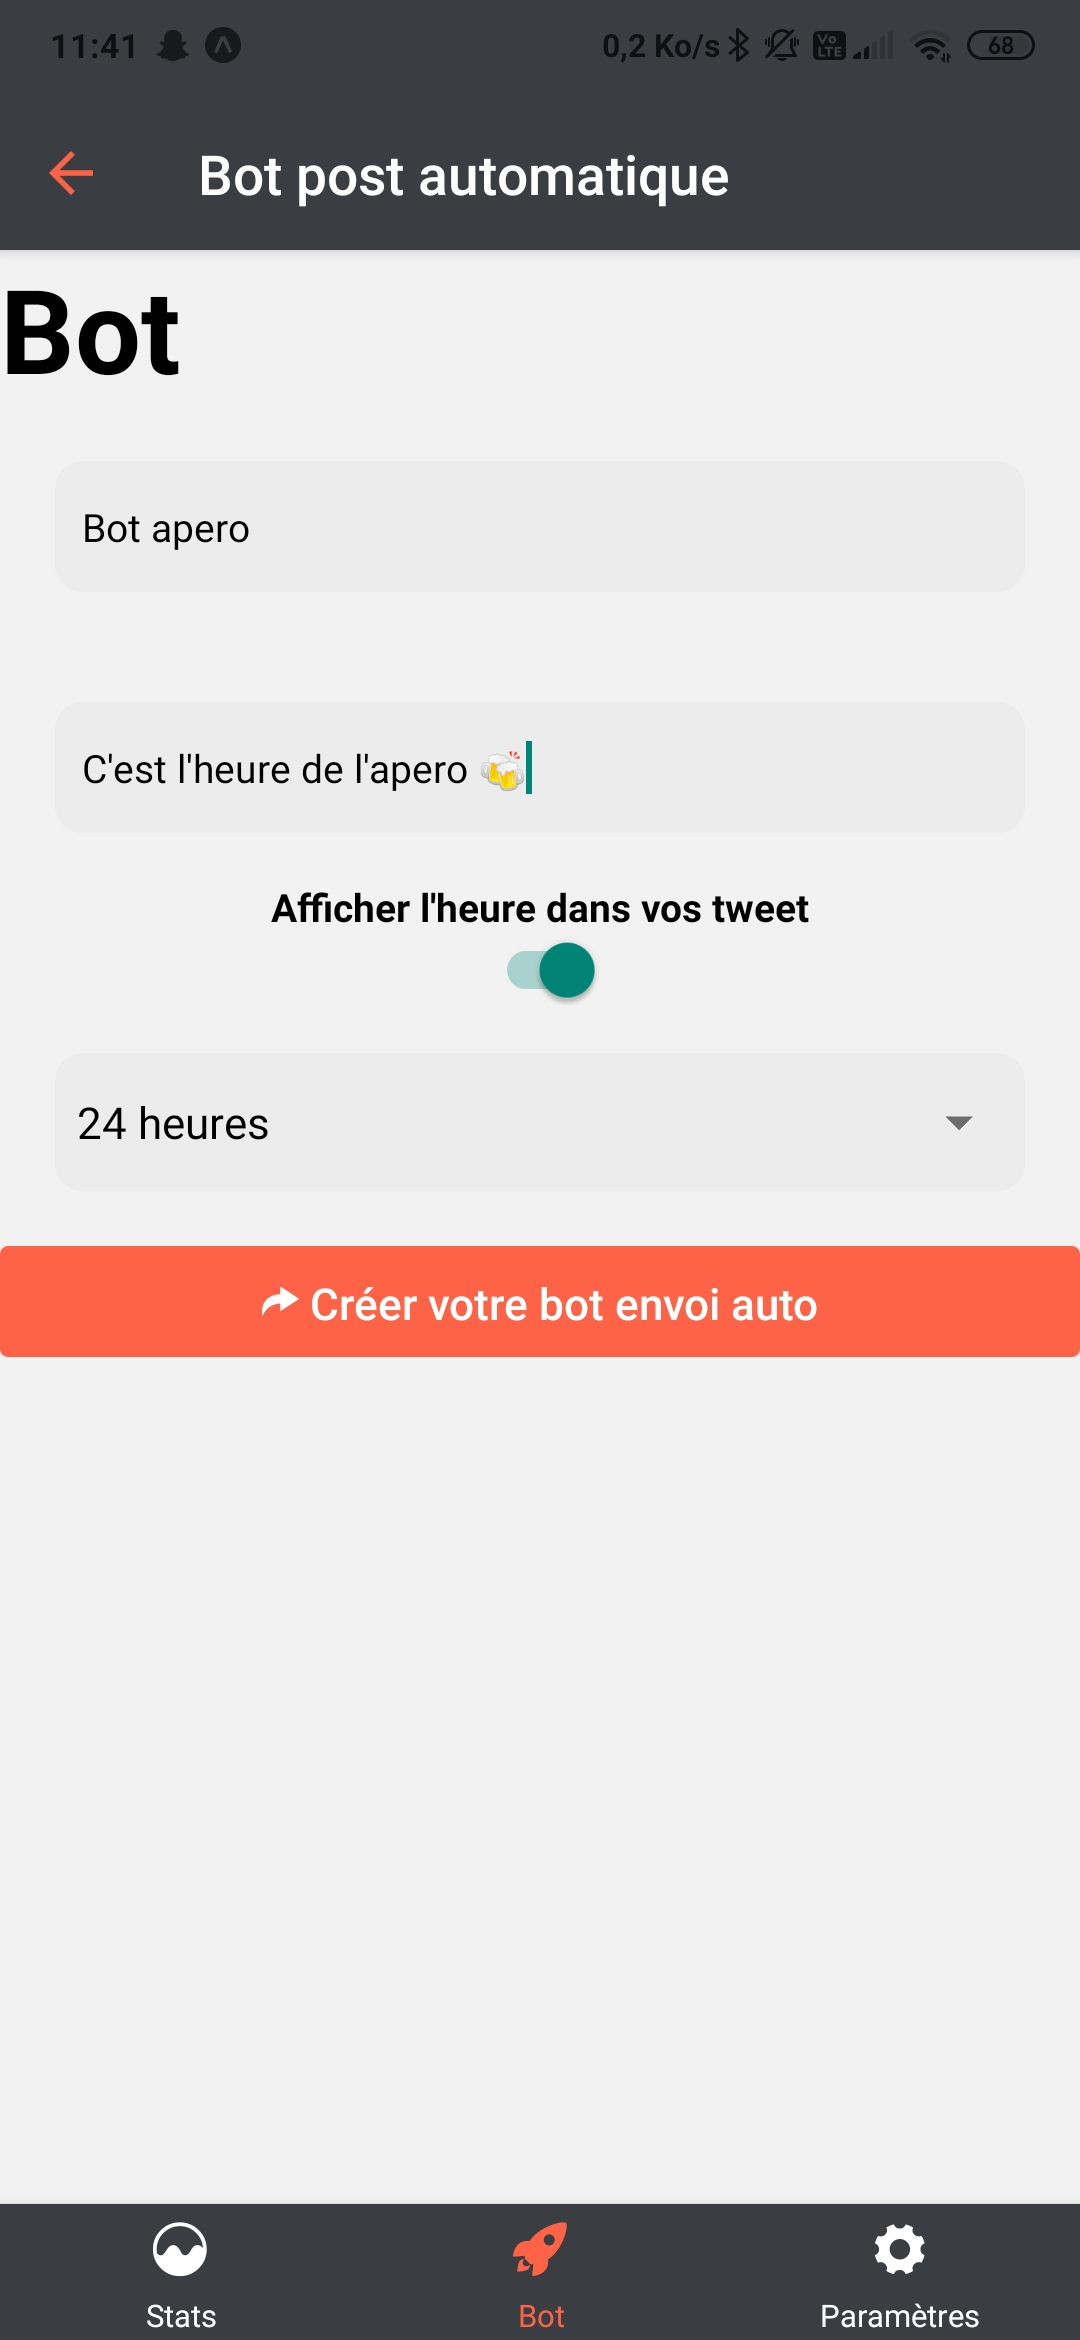
\includegraphics[scale=0.1]{images/crea_bot_post.jpg}
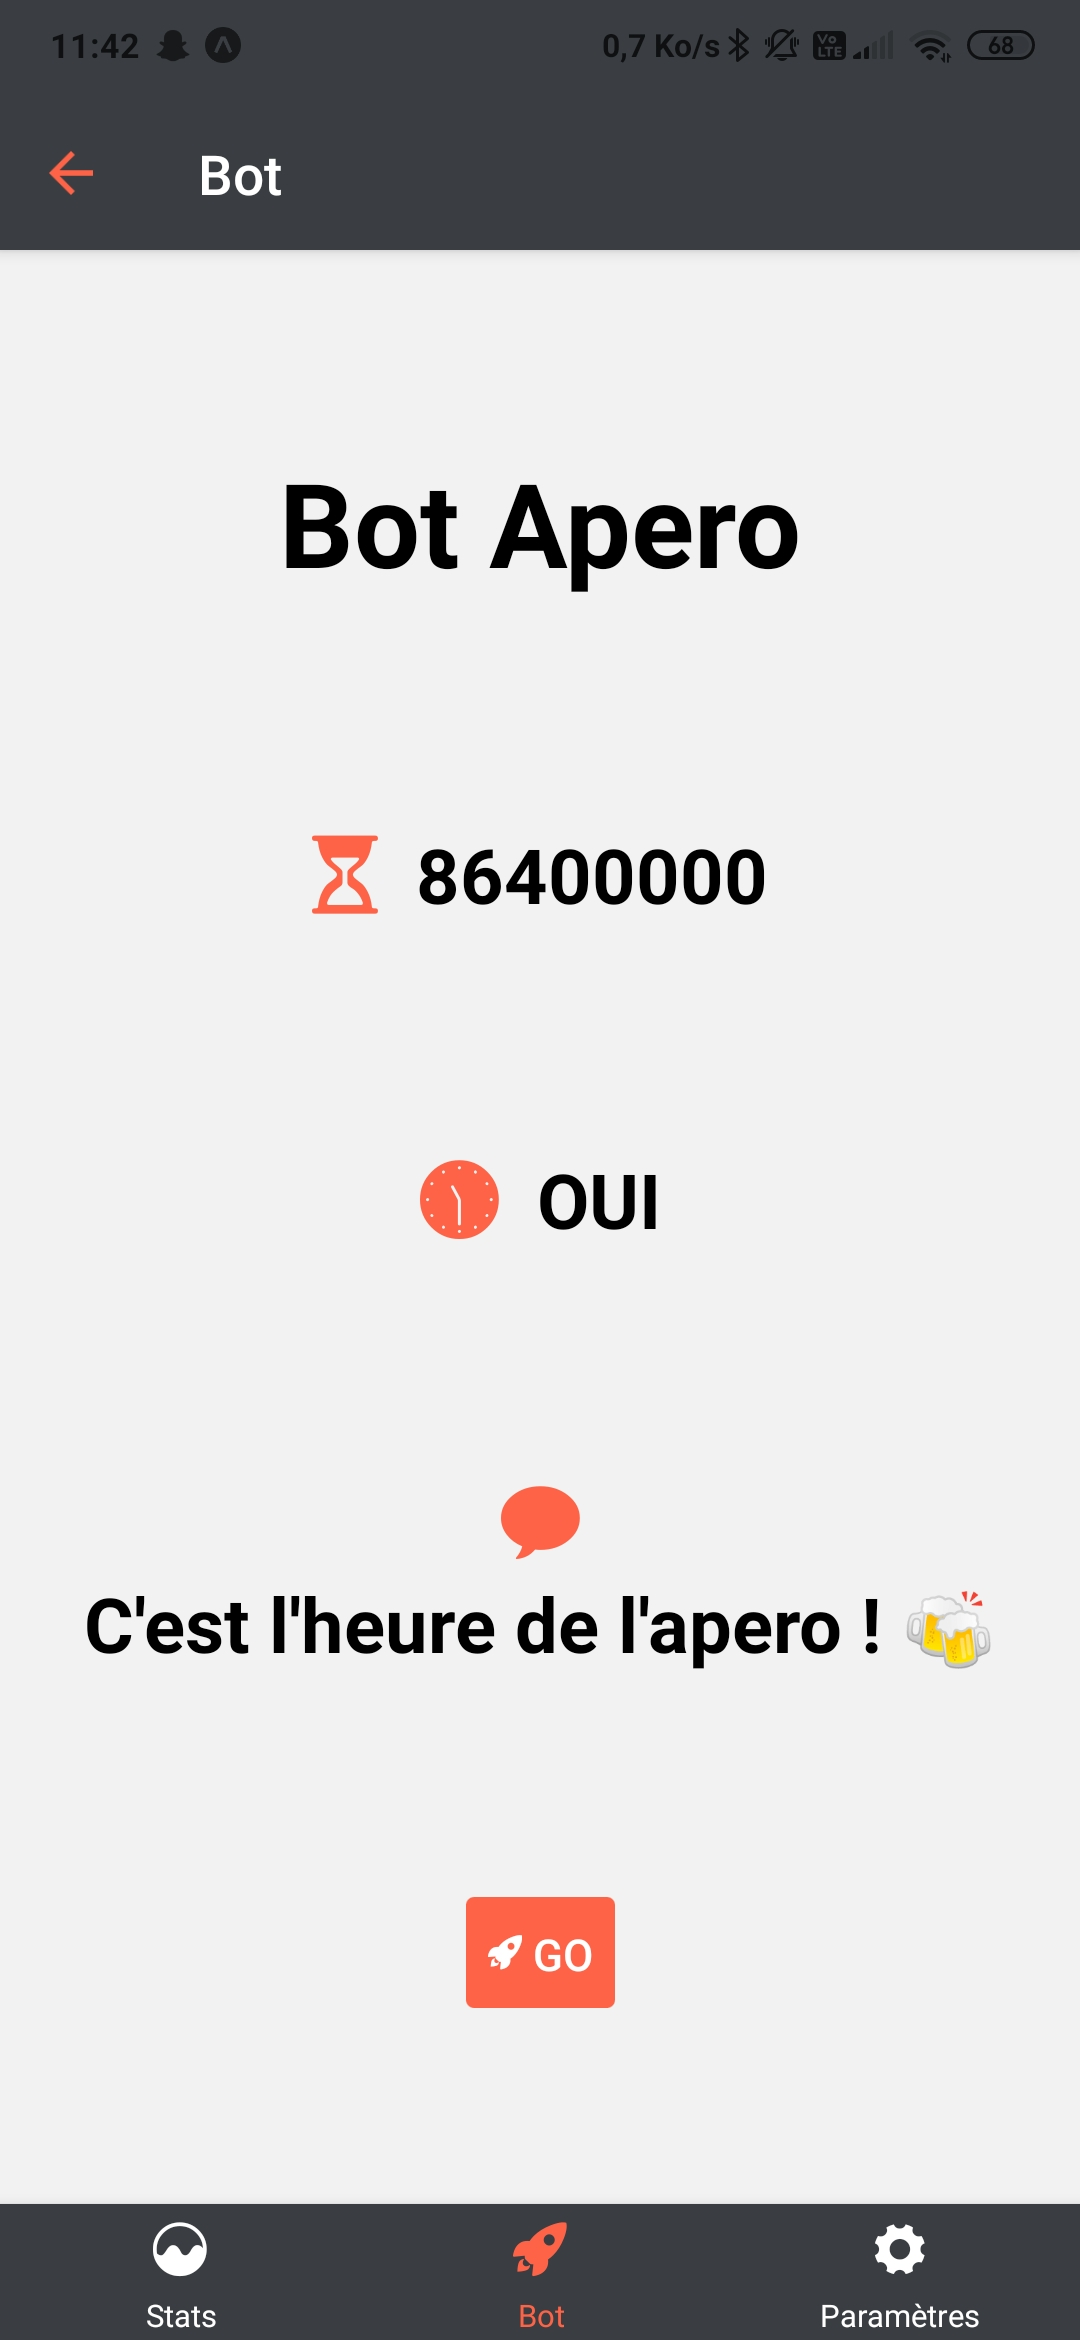
\includegraphics[scale=0.1]{images/recap_bot.jpg}
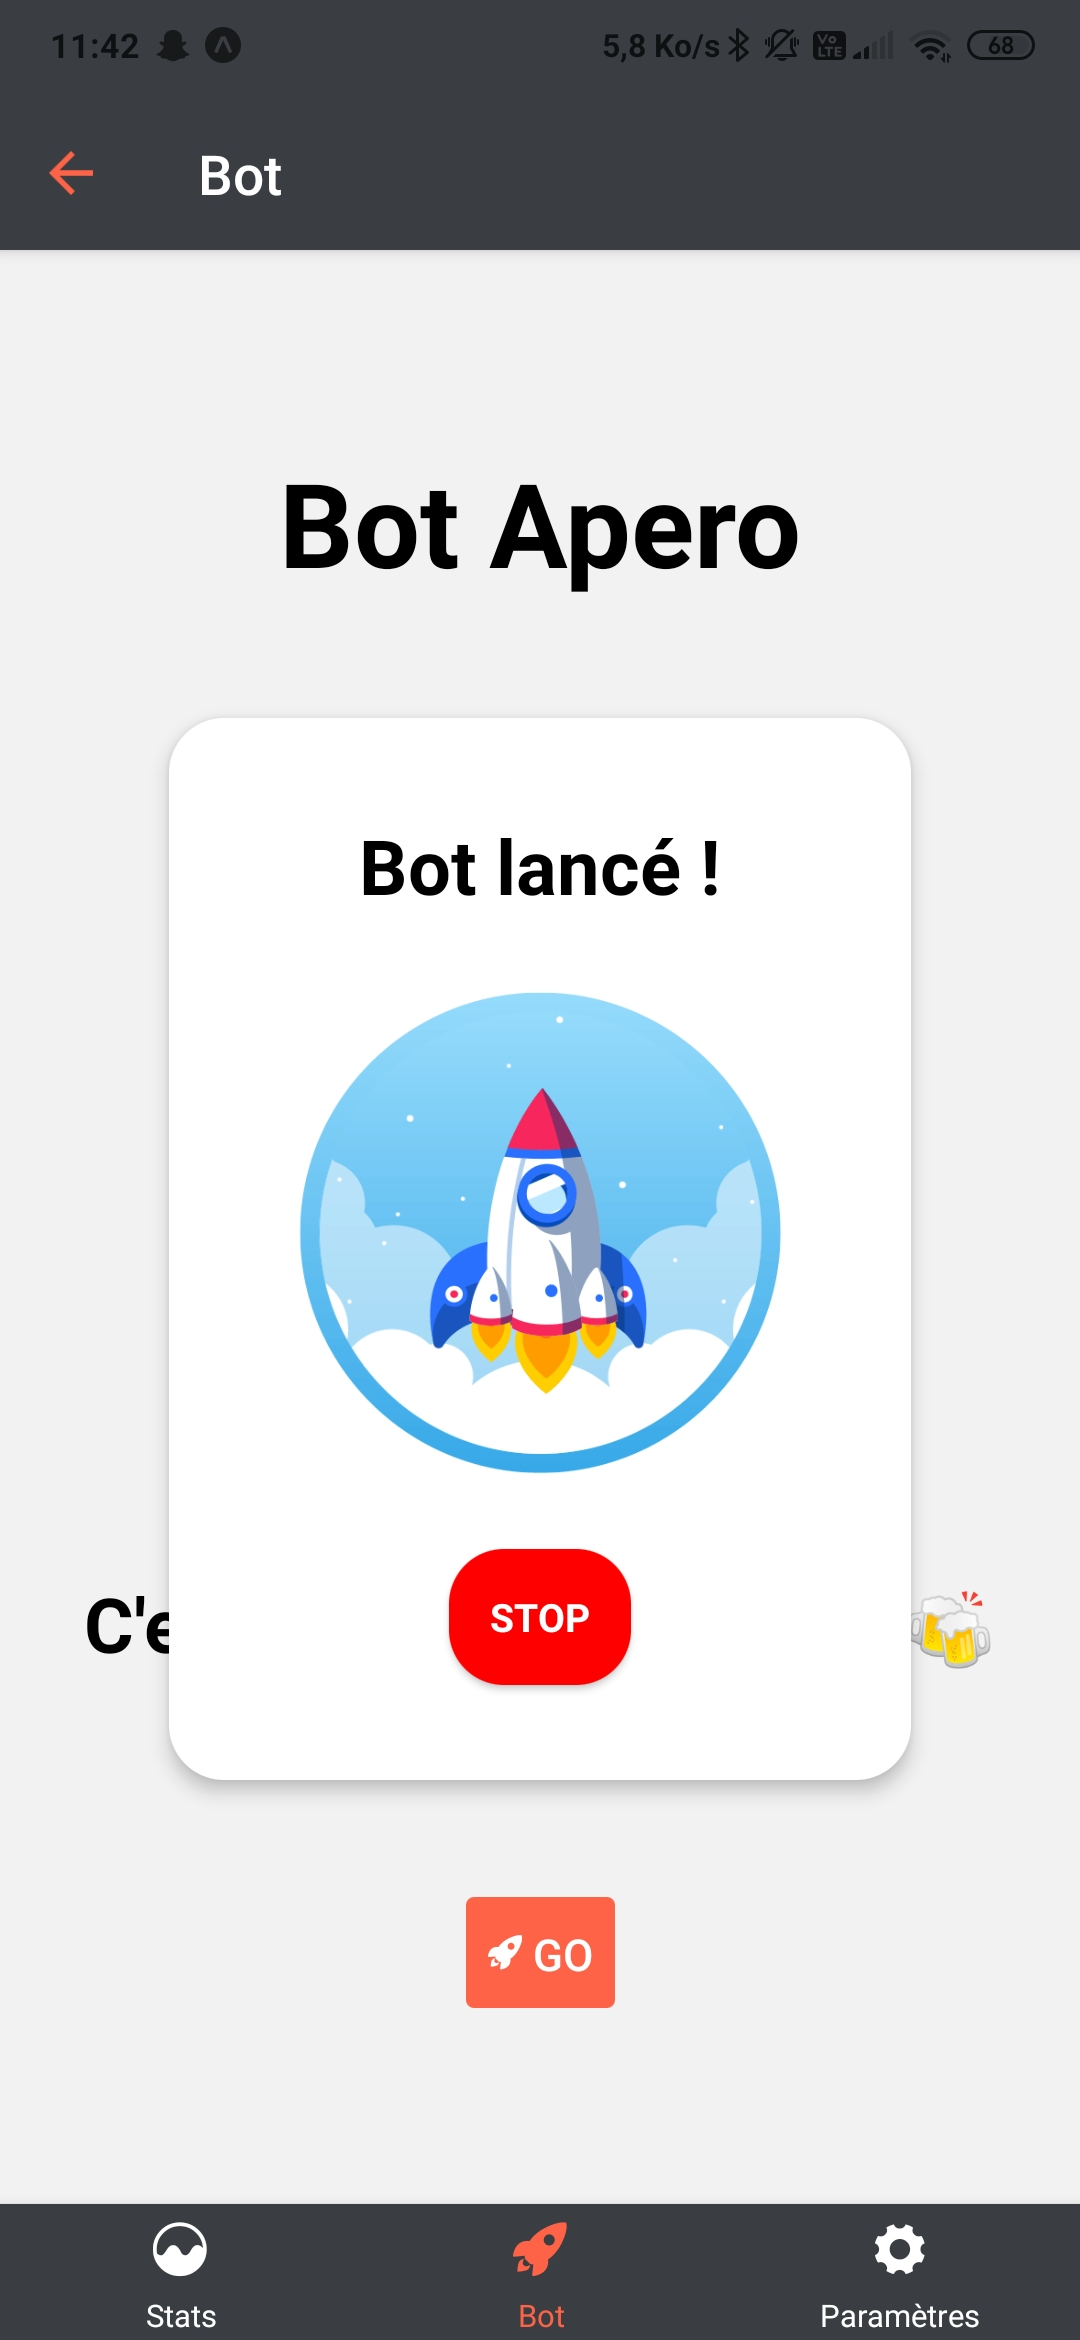
\includegraphics[scale=0.1]{images/lancement_bot.jpg}
\caption{Processus de création d'un bot de post automatique}
\label{fig:Processus de création d'un bot de post automatique}
\end{figure}

\subsubsection{Bot de réponses automatiques}
Pour ce qui est des bots de réponses automatiques aux mentions twitter, nous retrouvons comme précédemment un nom pour le bot, celui-ci sera utilisé pour le retrouver dans la liste des bots de l'utilisateur. Ensuite, nous avons fait le choix (dans un premier temps) de laisser à l'utilisateur 3 couples mots déclencheurs / réponse. Le nombre de 3 couples a été choisis afin de faciliter au plus le développement de l'application.
\newline\newline
Enfin, comme pour le précédent bot, l'utilisateur clique sur celui qu'il souhaite dans la liste, un écran récapitulant les informations du bot apparaîtront, puis le lance en appuyant sur le bouton "GO". Une animation se lance indiquant à l'utilisateur que le bot est lancé.

\begin{figure}[h!]
\centering
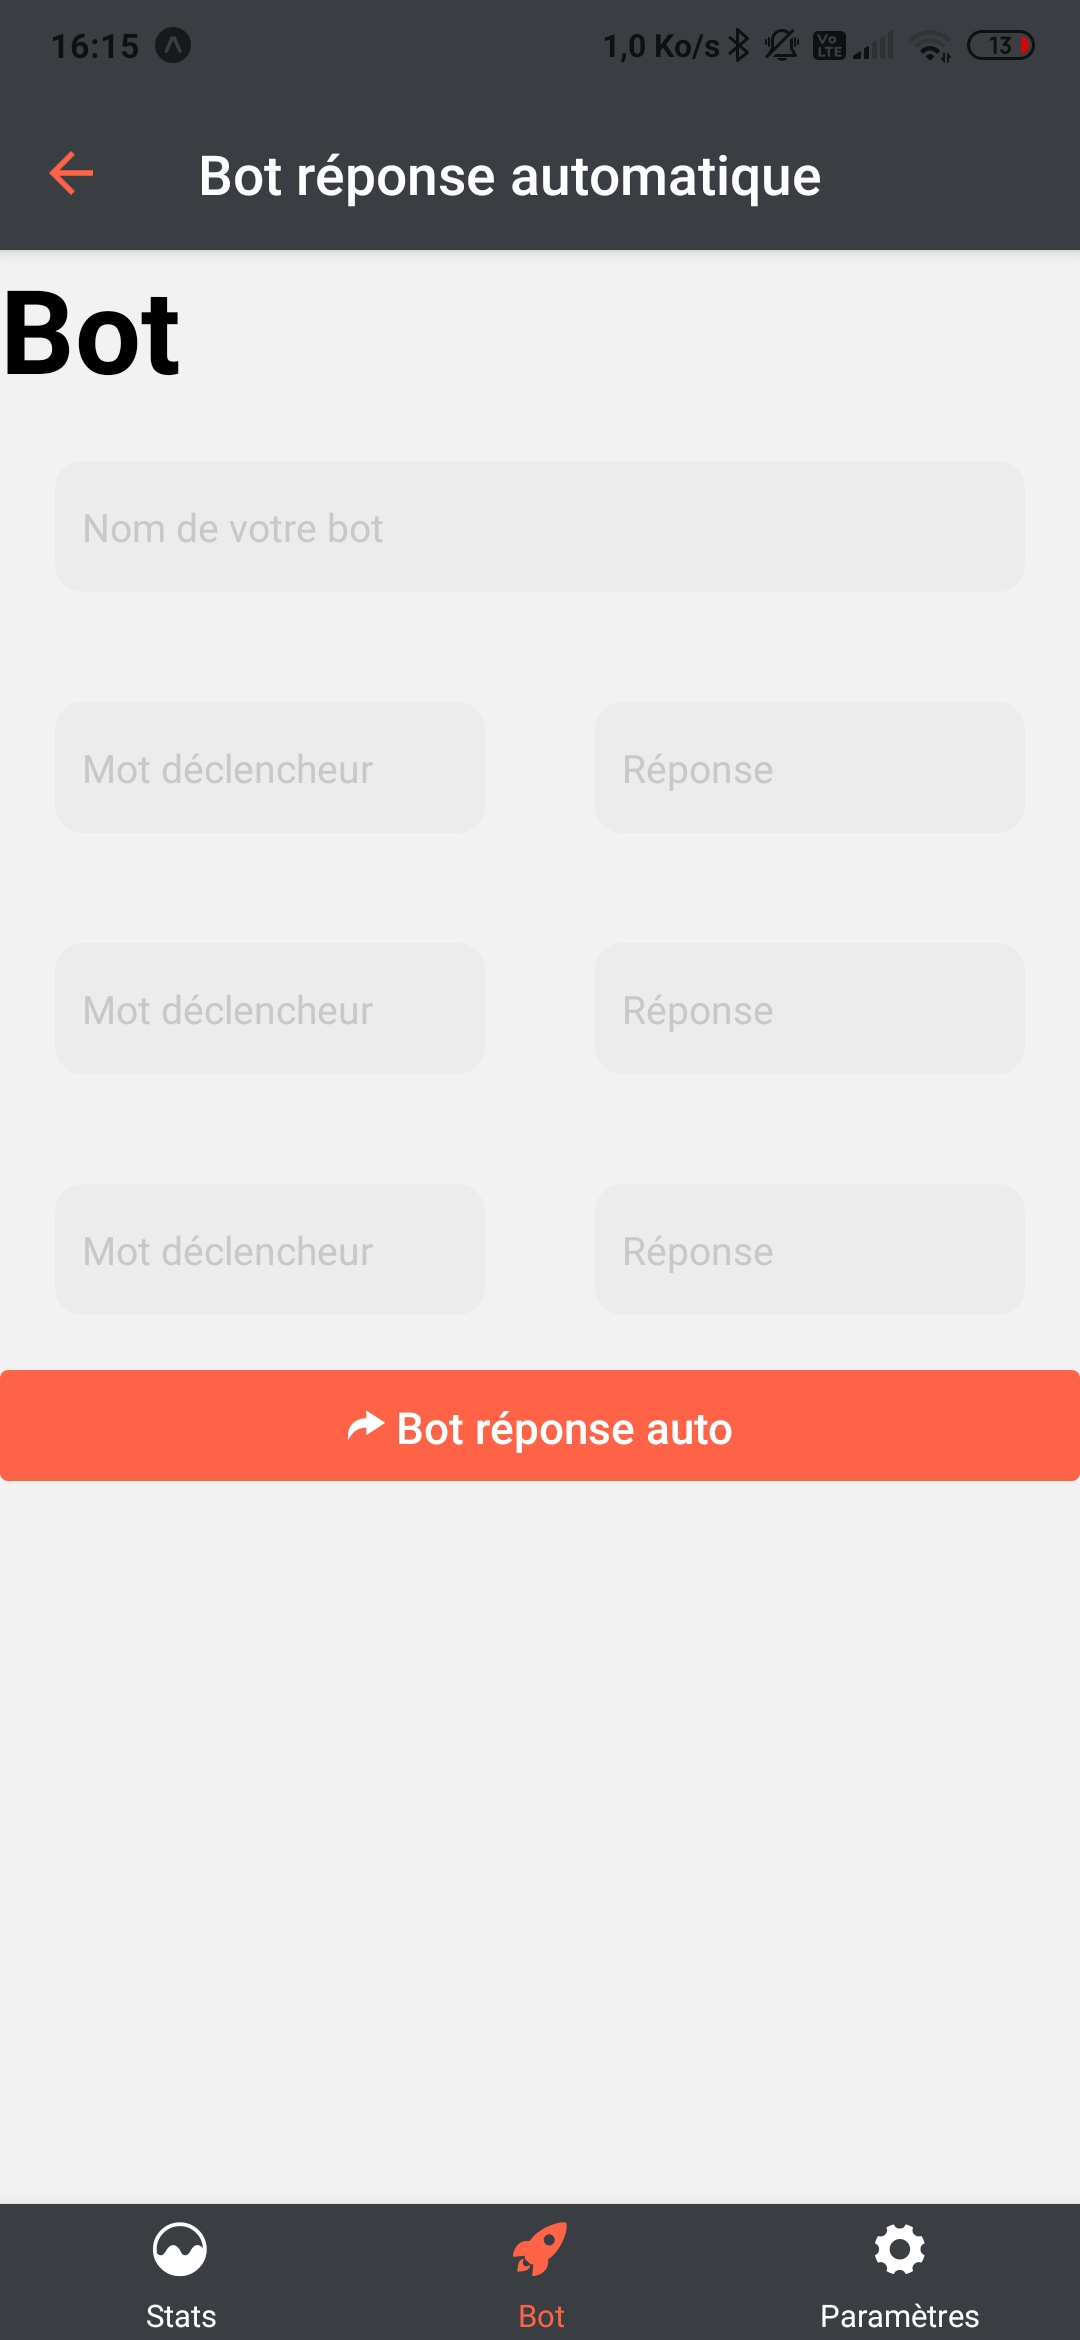
\includegraphics[scale=0.1]{images/crea_bot_reponse.jpg}
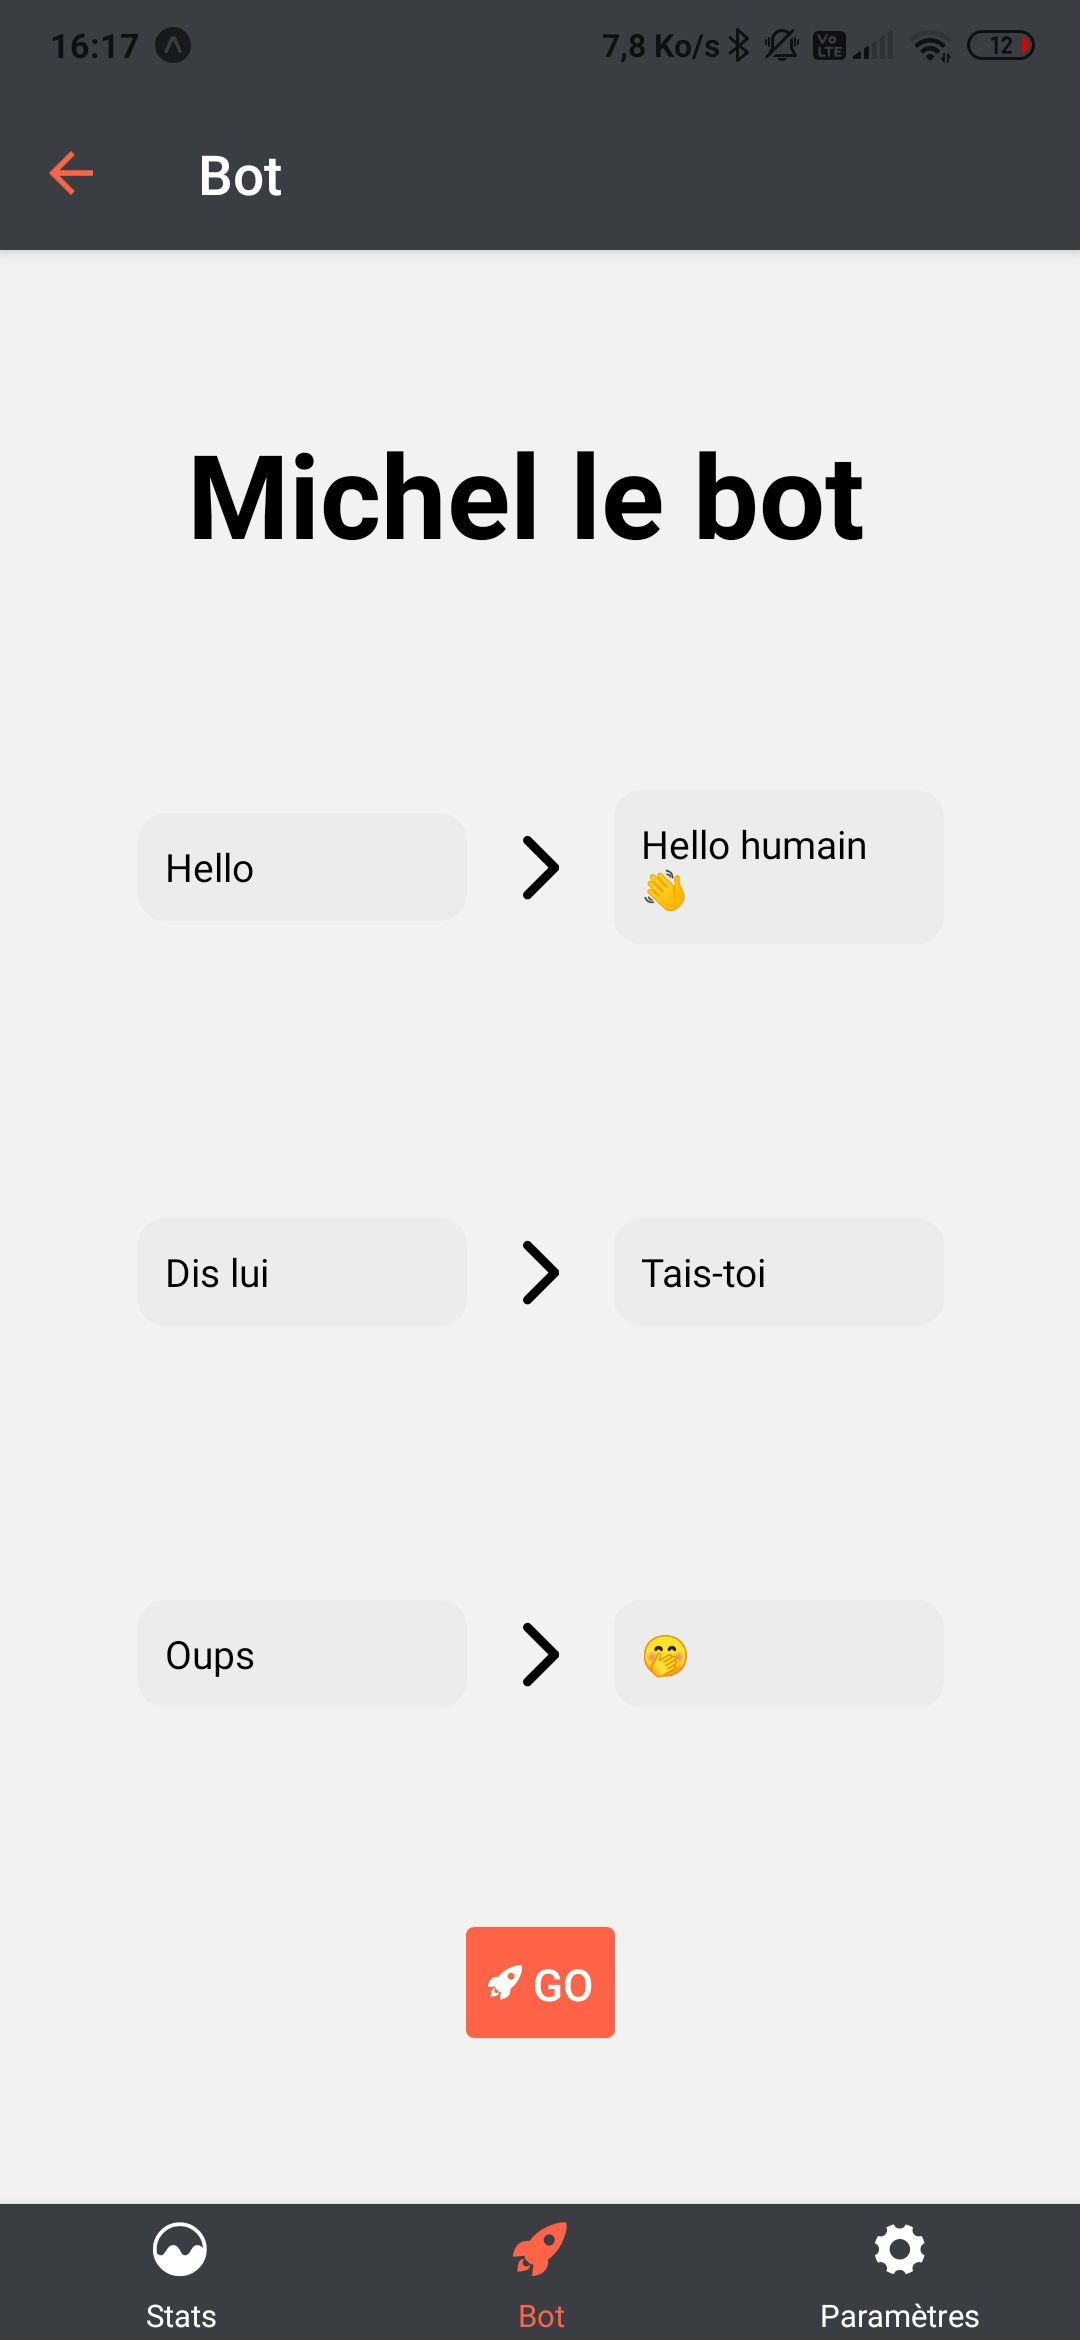
\includegraphics[scale=0.1]{images/recap_bot_reponse.jpg}
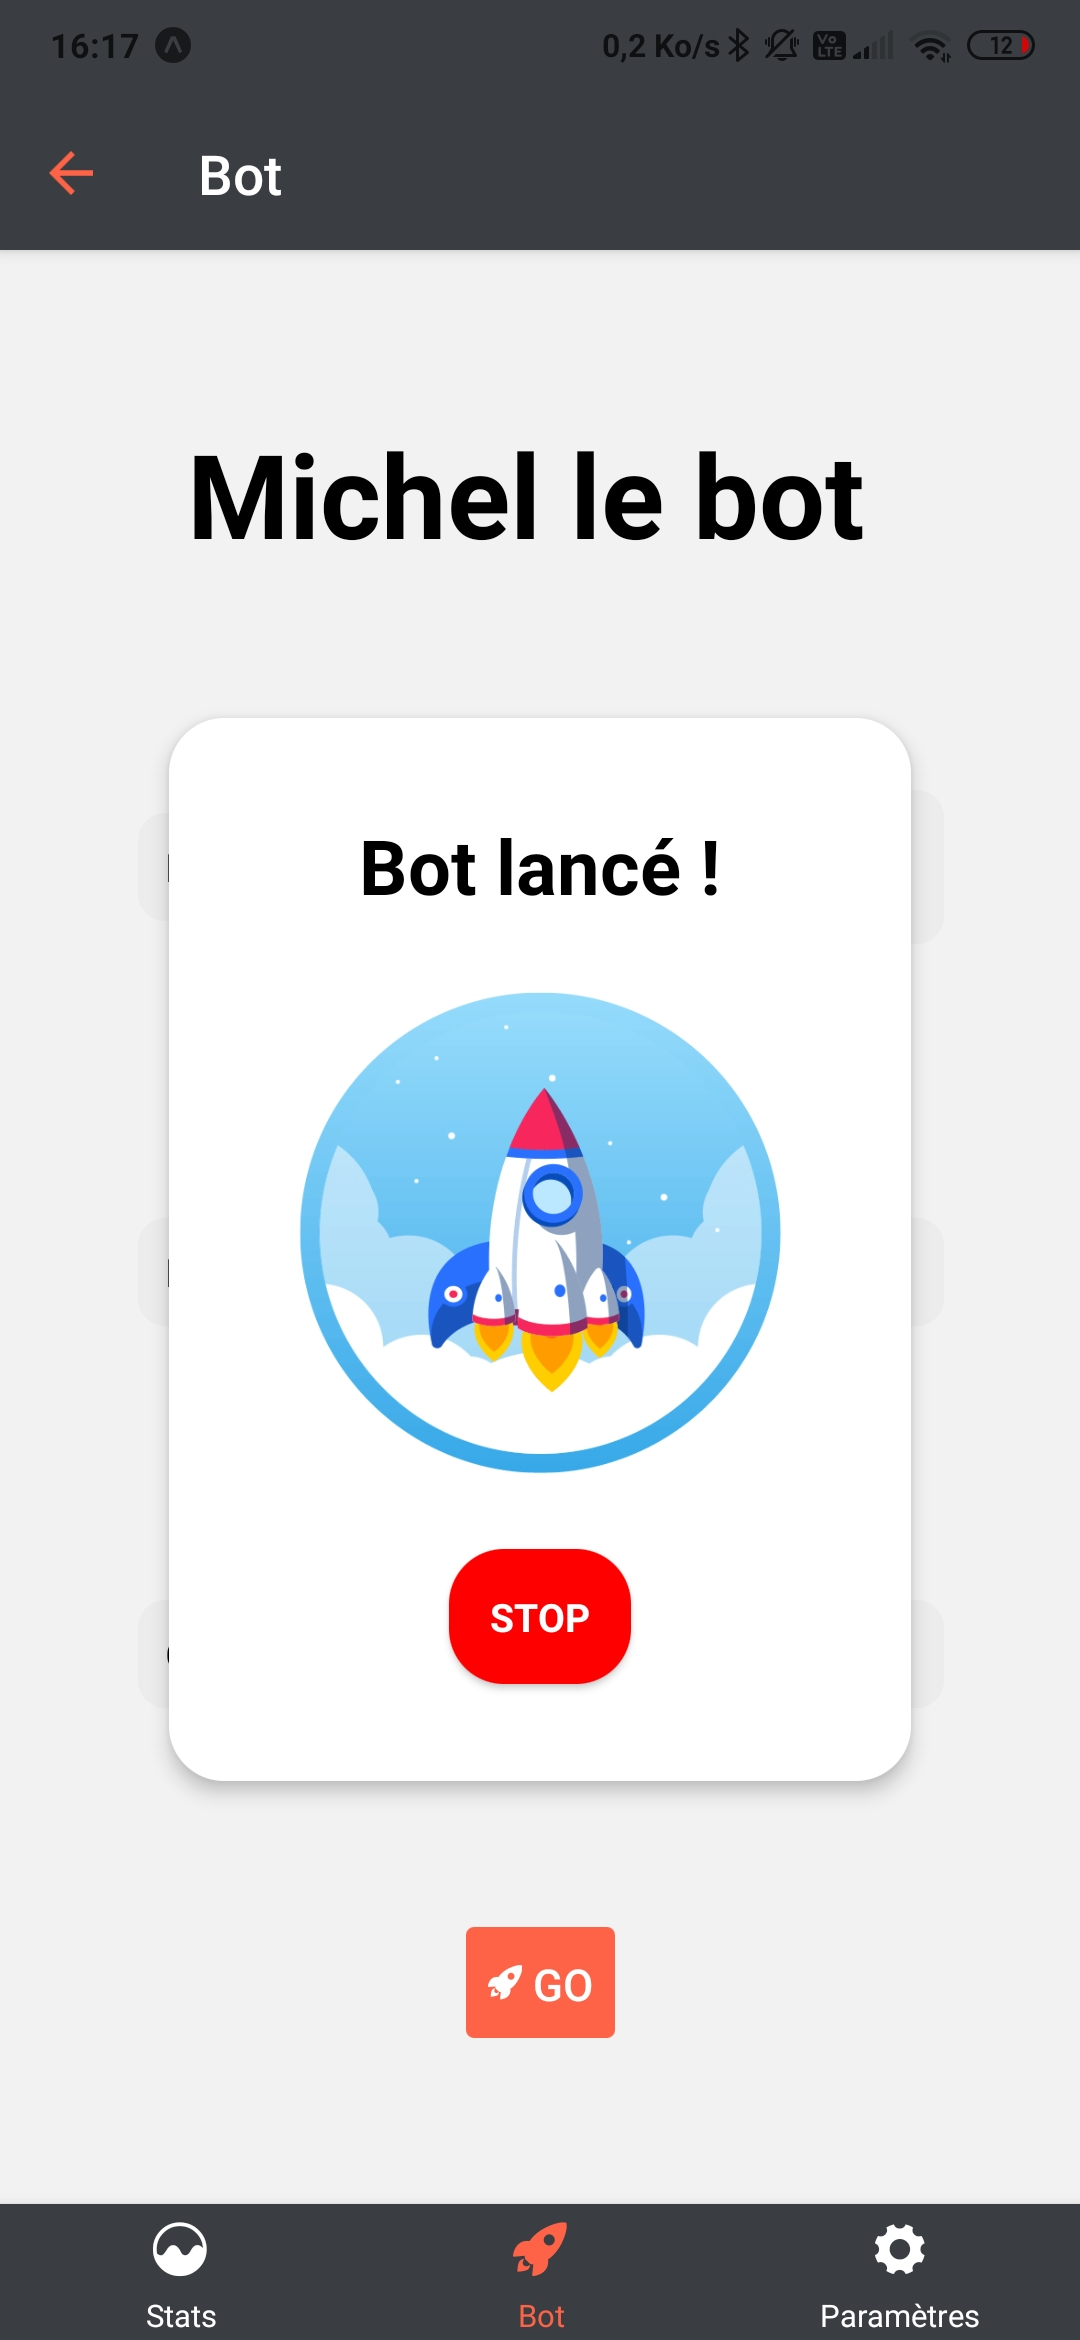
\includegraphics[scale=0.1]{images/lancement_bot2.jpg}
\caption{Processus de création d'un bot de réponses automatiques}
\label{fig:Processus de création d'un bot de réponses automatique}
\end{figure}

\newpage

\subsection{Développement des statistiques utilisateurs (réalisé par Bastien L.)}
L'application permet de retrouver un utilisateur twitter puis afficher quelques statistiques à propos de celui-ci. Dans le menu 'Stats' de l'application, nous retrouvons la liste des comptes favoris de l'utilisateur. Ceux-ci sont sauvegardés grâce l'utilisation de la librairie Redux \citep{redux}.
\begin{figure}[h!]
\centering
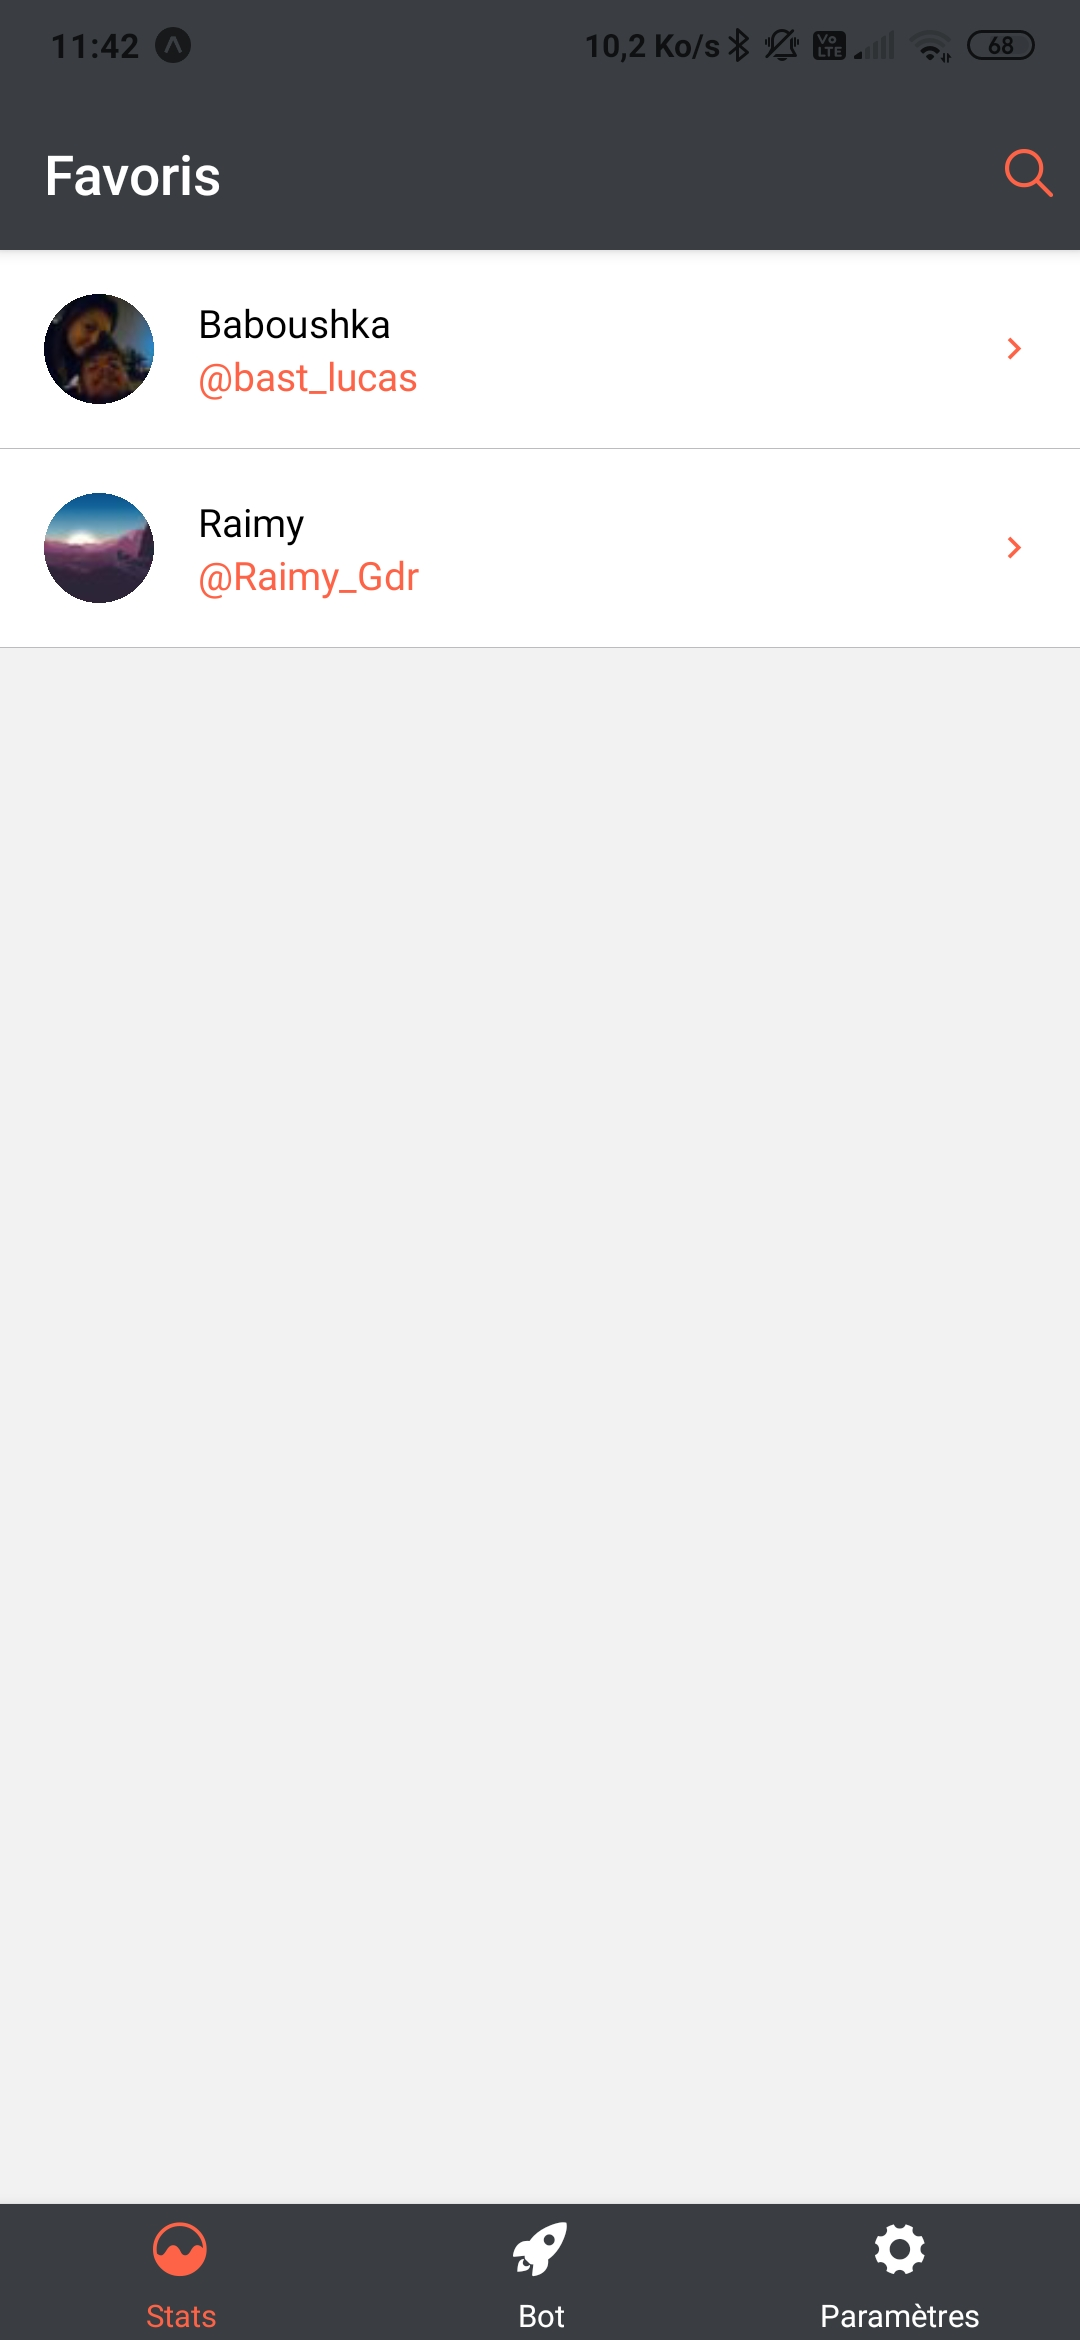
\includegraphics[scale=0.1]{images/liste_user.jpg}
\caption{Liste des utilisateurs enregistrés}
\label{fig:Liste des utilisateurs enregistrés}
\end{figure}
\newline\newline
Lorsque nous choisissons un utilisateur nous retrouvons les statistiques suivantes : la date de création de son compte, le nombre de tweets posté de puis sa création ainsi que son nombre de followers et abonnements. En haut à droite de l'écran se trouve une étoile, celle-ci permet d'ajouter (ou supprimer) un compte à ses favoris.

\begin{figure}[h!]
\centering
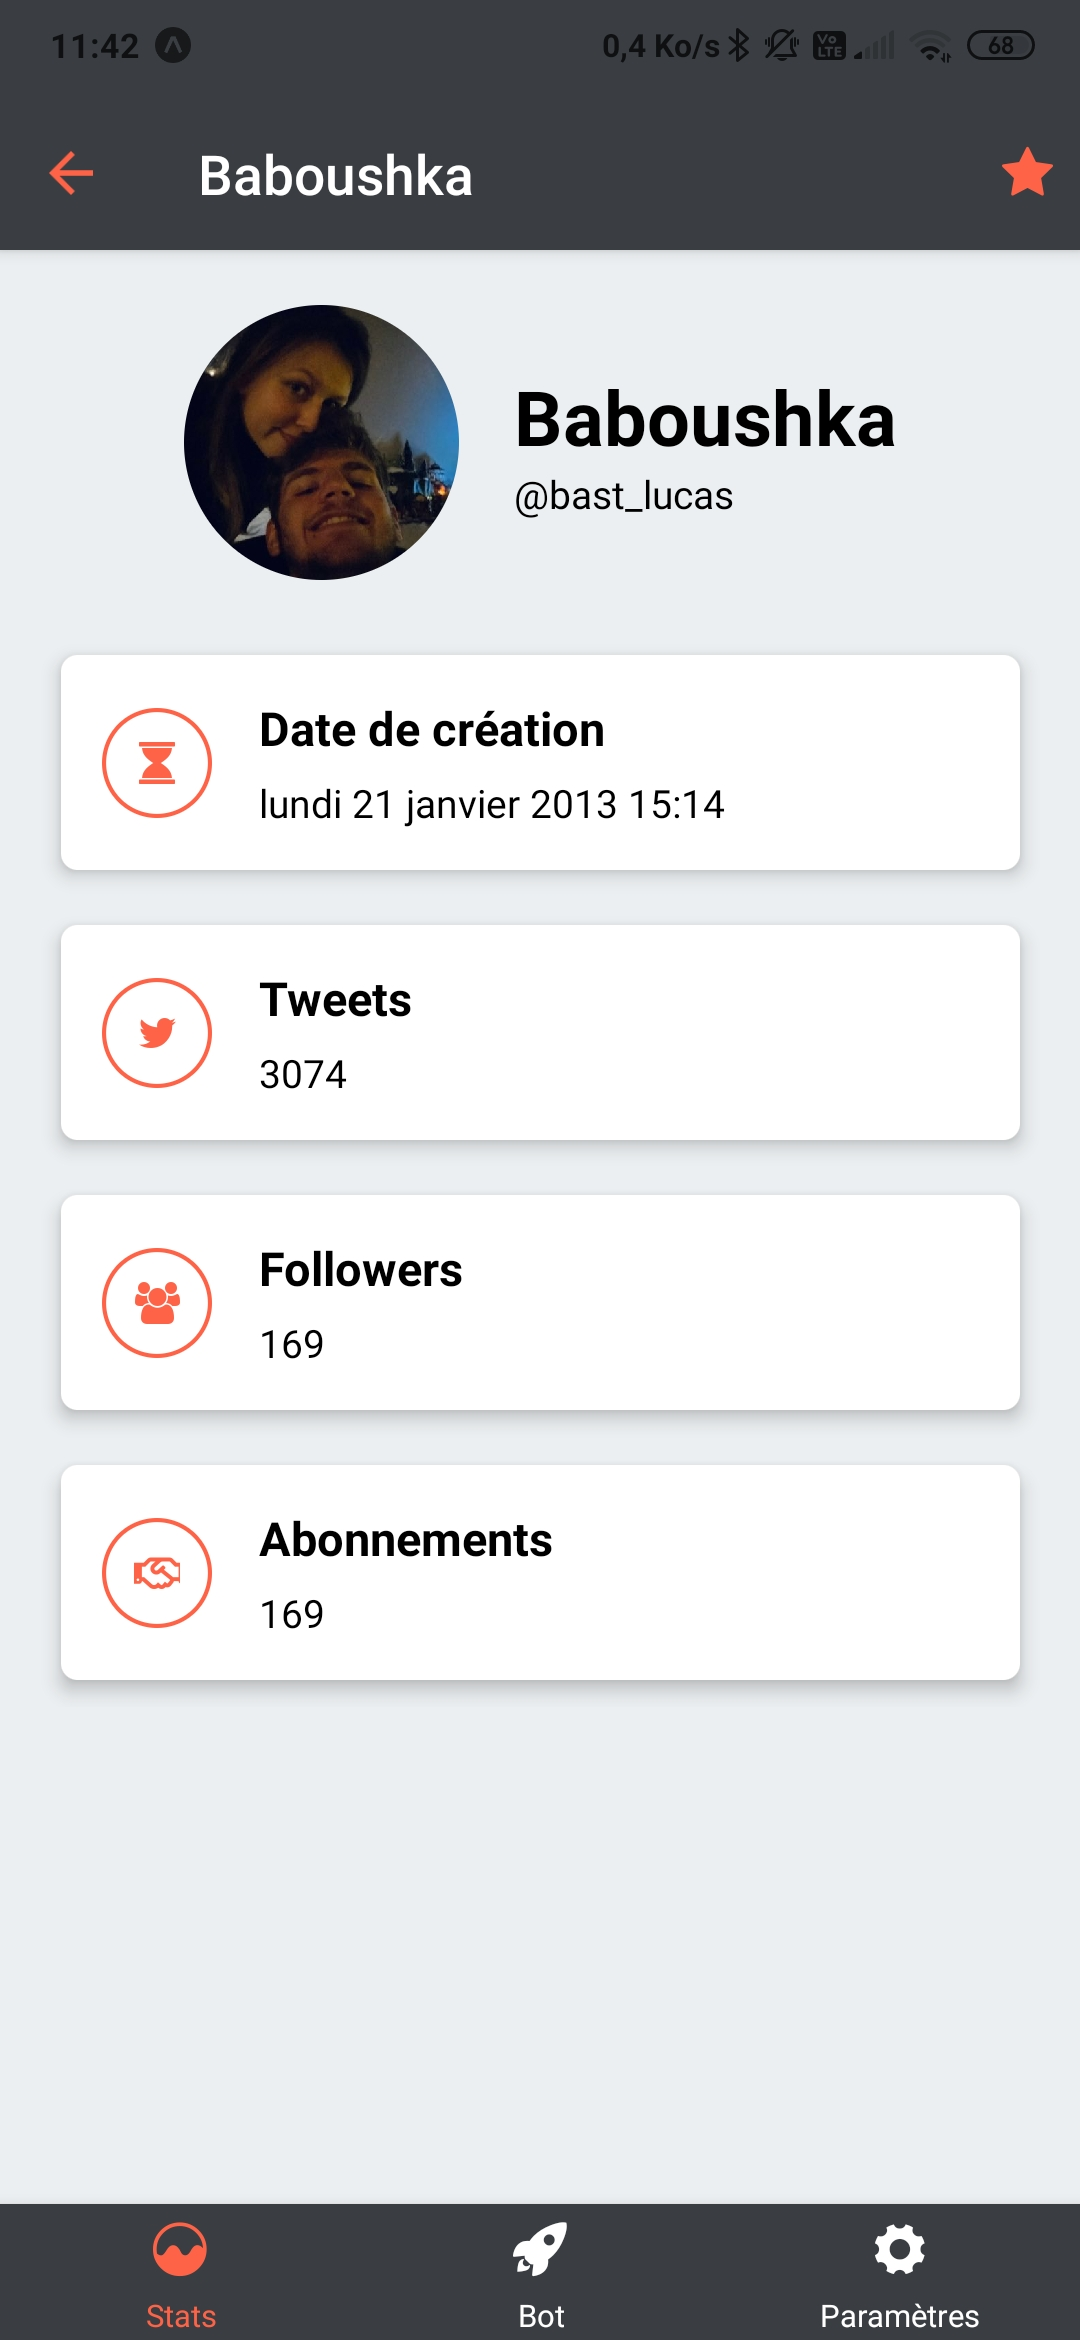
\includegraphics[scale=0.1]{images/stats_user.jpg}
\caption{Statistiques d'un utilisateur sur twitter}
\label{fig:Statistiques d'un utilisateur sur twitter}
\end{figure}


\bibliographystyle{plain}
\bibliography{references}
\end{document}
